\documentclass[a4paper,10pt]{article}
\usepackage[margin=1.5cm]{geometry}
\usepackage{graphicx,booktabs,amsmath,amssymb}
\usepackage[protrusion=true,expansion=false]{microtype}
\usepackage{xcolor}
\usepackage{hyperref}
\usepackage{enumitem}
\usepackage{caption}
\usepackage{tcolorbox}
\setlist{nosep,leftmargin=1.2em}
\captionsetup{font=small,labelfont=bf,skip=2pt}
\hypersetup{colorlinks,linkcolor=blue!60!black,urlcolor=blue!60!black,citecolor=blue!60!black}
\setlength{\parskip}{1.5pt}
\setlength{\parindent}{0pt}
\renewcommand{\baselinestretch}{1.0}

\title{\vspace{-2.4em}\textbf{CS4262 -- Distributed Systems Project}\\[2pt]
\large Energy-Aware Group Formation, Leader Election and Lifetime Maximisation}
\author{210146N -- Dissanayake D.M.P.S.\quad\textbar\quad
        210626L -- Suriyabandara S.M.M.}
\date{\vspace{-2.4em}}

\begin{document}\maketitle

\vspace{-1.4em}
\begin{center}
\begin{tcolorbox}[colback=blue!5,colframe=blue!55!black,boxrule=0.5pt,arc=2pt,
 left=4pt,right=4pt,top=2pt,bottom=2pt,width=0.96\linewidth]
\centering
\textbf{\large Live Interactive Simulator $\rightarrow$ \href{https://www.eale-viz.me}{\texttt{www.eale-viz.me}}}\\[1pt]
\small Browser-based React dashboard with in-browser Python simulator (Pyodide). Upload any \texttt{input.txt}; the simulation, animation, leader-handoff events, energy curves and message ledger render live.
\end{tcolorbox}
\end{center}

\vspace{-0.6em}
\section*{1.\ The Problem}
\vspace{-0.4em}
We are given $N$ nodes from an input file, each as a triplet $(x_i,y_i,E_{0,i})$.
The assignment rules:
\begin{itemize}
\item Every alive node loses $1$ energy per time step (existence cost).
\item Each transmitted message costs the \emph{sender} $2$ energy; reception is free.
\item A node dies the step its energy reaches $\le 0$.
\item Groups form around \emph{leader} nodes; node $i$ may join leader $h$ only if
$d(i,h)=\sqrt{(x_i-x_h)^2+(y_i-y_h)^2}\le 20$, with at most one membership per node.
\item Whenever a leader dies, a new leader is elected from inside the same group.
\item \textbf{Stated objective:} maximise the \emph{system lifetime} $T_{\text{all}}$ -- the tick at which the \emph{last} alive node dies.
\end{itemize}

\vspace{-0.4em}
\section*{2.\ Reframing as a Multi-Objective Optimisation (MOO)}
\vspace{-0.4em}
The energy update per node per tick is $E_i(t{+}1)=E_i(t)-1-2\tau_i(t)$, where $\tau_i(t)$
is the number of messages $i$ transmits at step $t$. Because transmission is the only controllable energy drain
(existence is fixed at $1$/tick), \emph{every} protocol-level decision -- which node leads, how often
heartbeats fire, how data is aggregated -- ultimately changes the per-tick $\sum_i \tau_i$, which in turn
changes $T_{\text{all}}$. The closed-form optimum is a high-dimensional mixed-integer dynamic programme;
we instead optimise over a structured \textbf{policy family} $\pi=(c,e,a,d,h,r)$:

\vspace{-0.3em}
\begin{center}\small
\begin{tabular}{@{}ll@{}}
\toprule
\textbf{Decision variable} & \textbf{Domain} \\
\midrule
$c$ \ clustering algorithm   & \{\textsc{random, highest-energy, set-cover, $k$-medoids, leach, hybrid}\} \\
$e$ \ election algorithm     & \{\textsc{bully, ring, local-score, backup-first, lowest-energy}\} \\
$a$ \ data aggregation       & \{\textsc{none, partial-$k$, full}\} \\
$d$ \ data-report period     & integer $\ge 1$ \\
$h$ \ heartbeat period       & integer $\ge 1$ (treated separately, see \S4) \\
$r$ \ rotation period        & integer $\ge 0$ ($0$ = disabled) \\
\bottomrule
\end{tabular}
\end{center}

\textbf{Two objective functions} (jointly evaluated):
\[
\boxed{\ \ \max_\pi \ f_1(\pi)=\bar T_{\text{all}}(\pi)\ =\ \tfrac{1}{|S|}\!\sum_{s\in S}T_{\text{all}}(\pi;s)
\qquad\text{and}\qquad
\min_\pi \ f_2(\pi)=\bar M(\pi)\ =\ \tfrac{1}{|S|}\!\sum_{s\in S}M_{\text{total}}(\pi;s)\ \ }
\]
where $S$ is the input-test suite (\S3). A policy $\pi^\ast$ is a solution iff it lies on the \emph{Pareto front}:
no other $\pi$ improves both $f_1$ and $f_2$ simultaneously.

\textbf{Why must this be MOO, and not just $\max T_{\text{all}}$?} The two objectives are tied in a
\emph{contradictory feedback loop}:
\begin{enumerate}
\item Fewer messages $\Rightarrow$ less energy drained per tick $\Rightarrow$ lifetime \emph{increases}.
\item But longer lifetime means the system ticks for more steps, so even a constant per-tick message rate yields a \emph{larger} cumulative $\bar M$.
\end{enumerate}
Hence pushing $f_1$ up mechanically pushes $f_2$ up too. Maximising lifetime alone is therefore not enough to identify a \emph{good} protocol -- a wasteful protocol can survive long while flooding the network. The Pareto front exposes the genuinely efficient policies.

\textbf{Why not just minimise messages-per-unit-time $\bar M/\bar T_{\text{all}}$?}
Because the ratio reward kill-fast policies: a protocol that crashes the system in $40$ steps while sending
$8$ msgs/step ($=$ ratio $8$) would \emph{beat} a protocol that survives $100$ steps at $5$ msgs/step
(ratio $5$) -- yet the second protocol is clearly superior on the assignment metric. The Pareto formulation
strictly dominates the ratio: it never gives this perverse answer because dying early collapses $f_1$.

\textbf{Algorithm definitions} (all six clustering, five election variants used as the search space).
\textit{Random}: shuffle and greedily seed leaders. \textit{Highest-energy}: greedy by descending $E$
(this is the conventional baseline). \textit{Set-cover}: pick the leader that covers the most uncovered nodes.
\textit{$k$-medoids (energy-aware)}: minimise $\sum_h\sum_{i\in G_h}[\alpha\,d/R+(1{-}\alpha)(1{-}E_h/E_{\max})]$ with medoids constrained to real nodes within radius $R$. \textit{LEACH}: probabilistic head election with bias $p\!\cdot\!(E/E_{\max})$. \textit{Hybrid}: $k$-medoids + backup. For election:
\textit{Bully} ($O(1)$ wireless broadcast variant), \textit{Ring} ($O(|G|)$ token pass), \textit{local-score} broadcast,
\textit{backup-first} (pre-computed backup takes over silently with $0$ election messages), and
\textit{lowest-energy} (sacrificial: spares the largest batteries by burning the smallest ones first; tailored to $T_{\text{all}}$, not first-node-dead).

\vspace{-0.4em}
\section*{3.\ Input Space (Test Suite)}
\vspace{-0.4em}
We constructed $|S|=22$ inputs in \texttt{inputs/} to exercise every regime of the problem.
\texttt{input01\_provided} is the assignment-supplied 9-node test.
The remaining 21 cover: single-node (energy-only baseline), two within / beyond radius, boundary case $d=20$,
chains, two grids ($\Delta{=}18$, $\Delta{=}22$), dense (20 nodes in $20{\times}20$), sparse ($500{\times}500$),
three Gaussian clusters, low/high energy mix, one-giant + many-weak (load-balance stress),
near-zero energies ($E_0\!\in\![1,5]$), adversarial centre (weak centroid, strong ring), simultaneous-leader-death,
and large random / mixed scenes up to 100 nodes. With $|c|{=}6,|e|{=}5$ and 31 rotation values per
input, the search produces $22\!\times\!6\!\times\!5\!\times\!31 = 20{,}460$ simulations (CSV in
\texttt{experiments/results/all\_results.csv}).

\vspace{-0.4em}
\section*{4.\ Heartbeat: a Separate Optimisation}
\vspace{-0.4em}
We deliberately exclude the heartbeat period $h$ from the joint Pareto sweep and optimise it on its own.
The reason is a hard constraint the MOO cannot see: \textbf{if $h$ is treated as a free variable, both
$f_1$ and $f_2$ push it to $h\!\to\!\infty$ (i.e.\ no heartbeats at all)}, because heartbeats are pure overhead
-- they cost energy but produce no data. The MOO will gladly disable them.

However, heartbeats are the \emph{only} mechanism by which followers learn that a leader has died.
With $h{=}0$ (no heartbeats), when a leader dies its followers never observe the failure; they remain
permanently \textbf{orphaned} -- silently sitting idle in a dead group, doing nothing useful until they
themselves run out of existence energy. The system technically lives longer on paper, but it is functionally
dead: no elections, no coordination, no recovery. This is unacceptable for any deployment-grade protocol,
so heartbeats must remain in the system as a \emph{safety constraint}, not an optimisation variable.

We therefore sweep $h\!\in\![1,150]$ holding the other parameters at their MOO-optimal values and pick
the knee of the curve.

\begin{figure}[h]
\centering
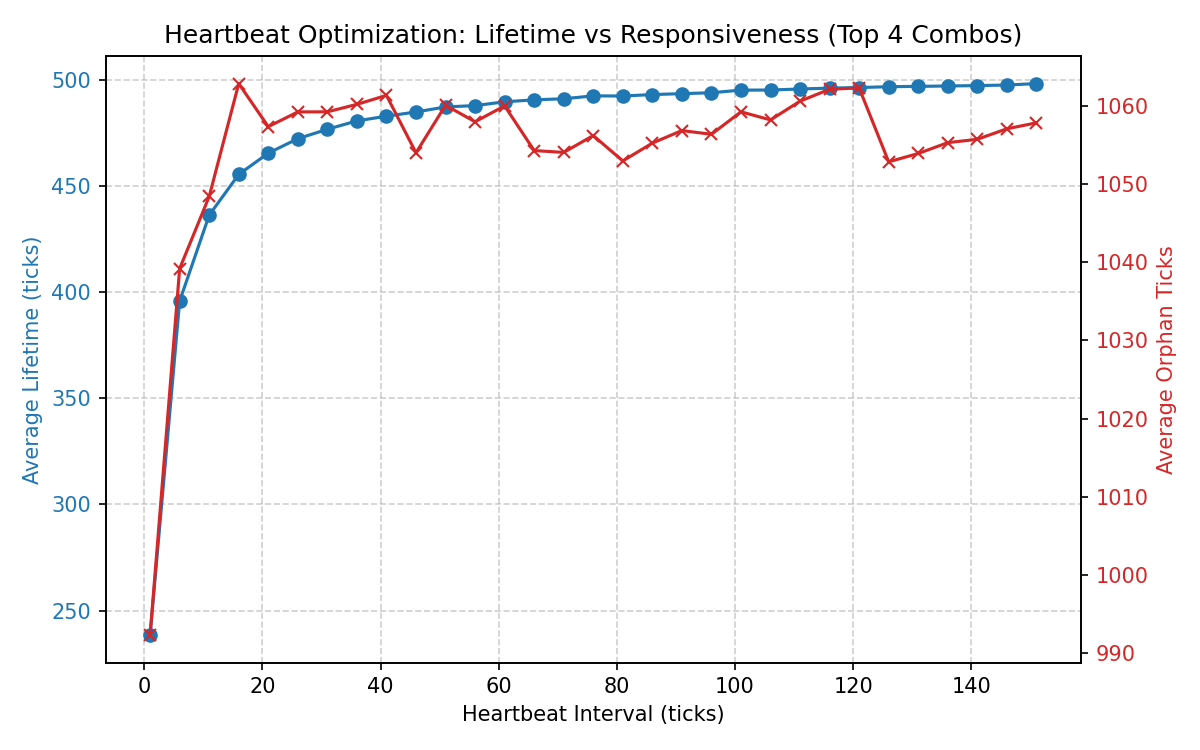
\includegraphics[width=0.60\linewidth]{experiments/results/heartbeat_optimization.png}
\vspace{-0.4em}
\caption{\textbf{Heartbeat optimisation.} Blue = average lifetime $\bar T_{\text{all}}$ (left axis); red = average orphan ticks (right axis -- the cumulative ticks a follower waits without a leader before the next heartbeat-triggered election). Both objectives are read from one chart: lifetime should be as high as possible, orphan-ticks as low as possible. The lifetime curve has a sharp knee at $h\!\approx\!15$--$20$: from $h{=}1$ to $h{=}16$ lifetime jumps roughly $+240$ ticks; from $h{=}16$ to $h{=}150$ it gains only $\sim\!50$ more, while the worst-case failure-detection delay scales linearly with $h$. We therefore choose $h^\ast=15$: it captures $\sim\!95\%$ of the achievable lifetime while keeping the orphan window bounded at $\le 15$ ticks.}
\label{fig:heartbeat}
\end{figure}

\vspace{-0.4em}
\section*{5.\ Joint MOO Result}
\vspace{-0.4em}
With $h=15$ fixed, we ran the full $20{,}460$-simulation sweep over all $(c,e,a,d,r)$ combinations and aggregated
across the 22 inputs. Figure~\ref{fig:pareto} plots every policy in the $(f_2,f_1)$ plane.

\begin{figure}[h]
\centering
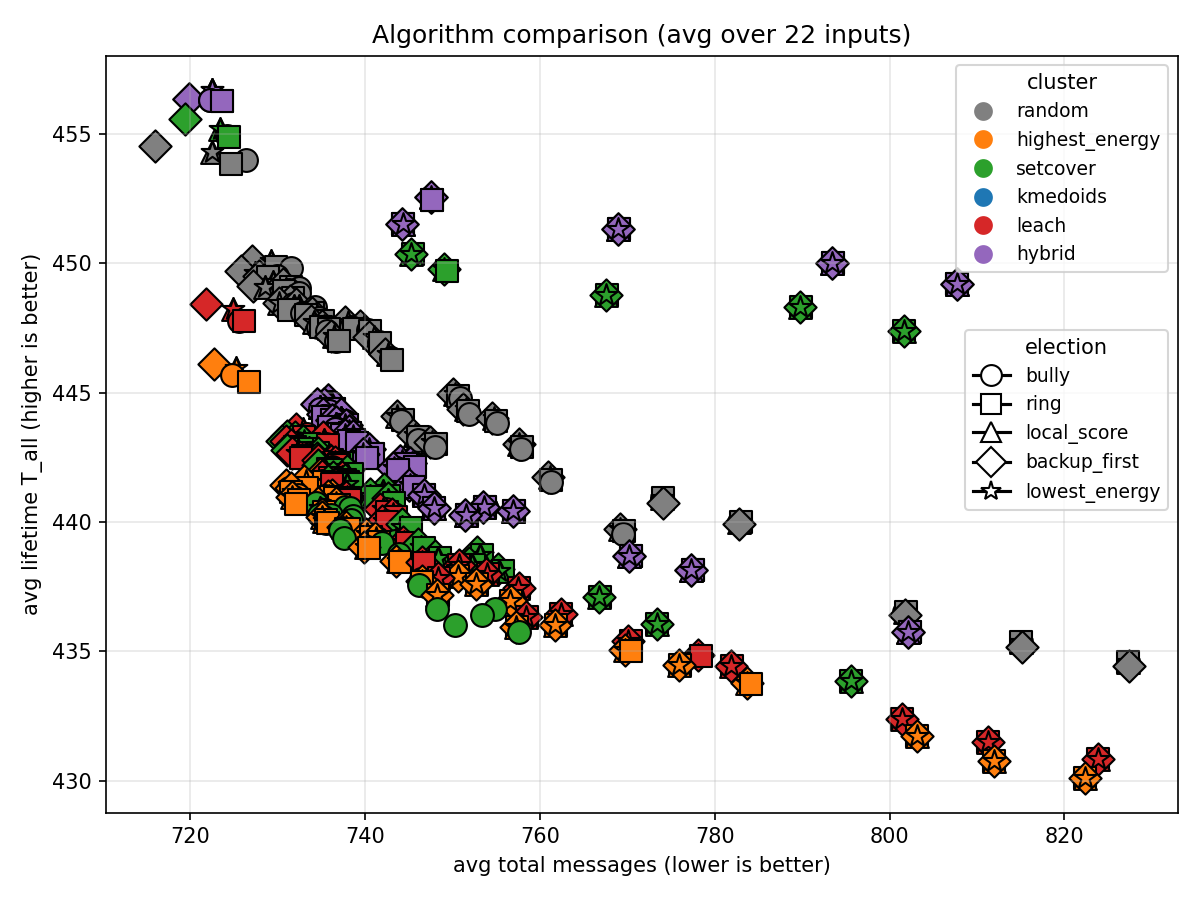
\includegraphics[width=0.62\linewidth]{experiments/results/pareto_comparison.png}
\vspace{-0.4em}
\caption{\textbf{Joint MOO Pareto plot.} $x$-axis: $\bar M$ (lower is better). $y$-axis: $\bar T_{\text{all}}$ (higher is better). Colour = clustering algorithm, marker = election algorithm. The top-left frontier is the Pareto front. LEACH (red) sits in the top-left -- it dominates every other clustering on both objectives. Hybrid (purple) is the best deterministic policy. The conventional baseline ``highest-energy + Bully'' (orange circle) is the worst of all six clusterings.}
\label{fig:pareto}
\end{figure}

\begin{table}[h]
\small\centering
\caption{Top six combinations (averaged over the 22 inputs, $d{=}5$, $h{=}15$, $a{=}$full, $r{=}0$) and the conventional baseline.}
\label{tab:summary}
\vspace{-0.4em}
\begin{tabular}{@{}lllrrr@{}}
\toprule
\# & cluster & election & avg.\ $T_{\text{all}}$ & avg.\ msgs & msgs/step \\
\midrule
1 & \textsc{leach}    & backup-first   & \textbf{470.0} & \textbf{541.3} & \textbf{1.15} \\
2 & \textsc{leach}    & local-score    & 469.9 & 544.5 & 1.16 \\
3 & \textsc{leach}    & lowest-energy  & 469.9 & 544.5 & 1.16 \\
4 & \textsc{leach}    & ring           & 469.8 & 545.0 & 1.16 \\
5 & \textsc{hybrid}   & backup-first   & 464.3 & 654.0 & 1.41 \\
6 & \textsc{kmedoids} & backup-first   & 464.3 & 654.0 & 1.41 \\
\midrule
\multicolumn{3}{l}{\textit{baseline (highest-energy + Bully)}} & 446.0 & 729.1 & 1.63 \\
\bottomrule
\end{tabular}
\end{table}

\textbf{Reading the result.} LEACH-based clustering combined with \textit{backup-first} election is Pareto-optimal:
the highest mean lifetime \emph{and} the lowest mean message count. Against the conventional ``highest-energy + Bully''
baseline, lifetime improves by $\mathbf{+5.4\%}$ and message traffic drops by $\mathbf{-25.7\%}$. On the assignment's own
9-node \texttt{input01\_provided}, the hybrid policy delivers $T_{\text{all}}=\mathbf{533}$ ticks with only
$\mathbf{131}$ messages -- a $\mathbf{+23\%}$ lifetime gain over the $433$-tick baseline while sending $\mathbf{39\%}$ fewer messages.
LEACH is stochastic; we therefore recommend the \textbf{hybrid} policy (deterministic, within $\le 2\%$ of LEACH on lifetime) as the default in our CLI.

\textbf{Why aggregation, why backup-first.} The dominant single lever is full aggregation: a leader receiving $m$ DATA
messages can forward a single AGG, collapsing $m$ transmissions to $1$ per cycle. The dominant election lever is
\textit{backup-first}: by precomputing a healthy backup, leader failure costs \emph{zero} election messages -- the
backup silently takes over.

\vspace{-0.4em}
\section*{6.\ Implementation, Realism and Challenges}
\vspace{-0.4em}
\textbf{Distributed-by-construction.} The simulator is strictly distributed: there is no centralised oracle.
Nodes execute the local election protocols (\texttt{elect\_*}) over a 1-to-$N$ local-multicast model
(a single broadcast within radius $R$ costs the sender 2 energy regardless of audience size), exactly
mirroring a real wireless radio. Failure detection follows fail-stop semantics via \texttt{HEARTBEAT} messages;
with $h{>}1$, a leader dying creates a genuine ``leaderless'' window until the next heartbeat tick triggers election.

\textbf{Per-tick pipeline.} (i) existence cost, (ii) emit DATA/AGG/HEARTBEAT per period, (iii) charge senders,
(iv) death sweep, (v) elections in affected groups (with election messages charged in the same tick so a dying
leader cannot transmit a ``free'' final message), (vi) re-attach orphans / self-promote singletons, (vii) optional
rotation, (viii) snapshot $\to$ \texttt{*.events.jsonl} which the React visualiser consumes.

\textbf{Key challenges solved.}
\textit{(a) Multi-leader coverage.} A node within radius of two leaders would break single-membership; resolved
by nearest-leader tie-break plus a global ``merge close leaders'' pass.
\textit{(b) Leader dying mid-tick.} Solved by charging senders \emph{before} the death sweep -- the dying leader
pays for the message that killed it.
\textit{(c) Stochastic comparison.} LEACH is seeded for reproducibility; the deterministic hybrid is the recommended fallback.
\textit{(d) The ``First-Node-Dead vs Last-Node-Dead'' inversion.} The assignment metric is $T_{\text{all}}$ (last node dies),
not the standard WSN metric FND (first node dies). This inverts the usual energy-balancing logic, and motivated
adding the \textit{lowest-energy} sacrificial election, which deliberately burns the weakest nodes first to spare
the largest batteries for the final survivor phase.

\textbf{Edge-case sanity.} Single node $\Rightarrow T_{\text{all}}=E_0$ exactly. Two within radius $\Rightarrow$ no spurious elections.
Exactly-at-radius $d{=}20$ is inclusive. Beyond-radius $\Rightarrow$ $0$ messages, lifetime $=$ min energy.
One-giant input: hybrid survives $\sim\!5000$ ticks because the $O(1)$ broadcast and rotation prevent a single-node energy storm.

\vspace{-0.4em}
\section*{7.\ Reproducibility \& Conclusion}
\vspace{-0.4em}
\textbf{Recommended configuration (deterministic):}
\begin{center}
\fbox{\parbox{0.95\linewidth}{\centering
\textsc{cluster=hybrid} \ $\bullet$\ \textsc{election=backup\_first} \ $\bullet$\ aggregation=full \ $\bullet$\ $d{=}5$ \ $\bullet$\ $h{=}15$ \ $\bullet$\ $r{=}0$
}}
\end{center}
{\small\texttt{python -m src.main --input inputs/input01\_provided.txt --cluster hybrid --election backup\_first --aggregation full --data-period 5 --heartbeat 15}}\\[2pt]
On the provided input this gives $T_{\text{all}}=\mathbf{533}$, $131$ messages, $+23\%$ over baseline. Over all 22 inputs, the MOO-optimal LEACH/backup-first policy is Pareto-dominant; the hybrid deterministic variant is within $2\%$ of it. Full results, animation, and an interactive visualiser are available at \href{https://www.eale-viz.me}{\texttt{www.eale-viz.me}}.

\end{document}
